\documentclass{rapport}
\usepackage[utf8]{inputenc}
\usepackage[T1]{fontenc} 
\usepackage{pifont} % Pour les symboles appelés par la macro \ding
\usepackage{url} % Comme son nom l'indique, pour les url...
\usepackage{amssymb}
\usetikzlibrary{positioning} % Bibliothèque tikz pour positionner des nœuds relativement à d'autres

\usepackage[colorlinks, citecolor=red!60!green, linkcolor=blue!60!green, urlcolor=magenta]{hyperref} % Pour que les liens soient cliquables. Les options permettent de mettre les liens en couleur.

\usepackage{mathrsfs}
\usepackage{pgfplots}
    
\usepackage{algorithm}
\usepackage{algo}
\usepackage{colorationSyntaxique}


% Pour un rapport en français 
\usepackage[french]{babel} % Commenter pour un rapport en anglais
\renewcommand\bibsection{\section*{Bibliographie}} % Commenter pour un rapport en anglais

% \englishTitlePage % Décommenter pour une page de titre en anglais


\pagestyle{fancy}
\renewcommand{\sectionmark}[1]{\markboth{\thesection.\ #1}{}}
\fancyfoot{}

\fancyhead[LE]{\textsl{\leftmark}}
\fancyhead[RE, LO]{\textbf{\thepage}}
\fancyhead[RO]{\textsl{\rightmark}}

\def\Latex{\LaTeX\xspace}
\def\etc{\textit{etc.}\xspace}



\title{Extraction automatique de ContextMaps dans des architectures micro-services}
\author{Thomas FARINEAU, Léo KITABDJIAN, Mohamed MAHJOUB}
\supervisor{Philippe COLLET}
\date{Second semestre de l'année 2023-2024}

 \universityname{Université Côte d'Azur} % Nom de l'université.
 \type{PER} % Type de document
 \formation{SI5 AL / M2} % Nom de la formation

% Retrouver les autres options possibles dans le document rapport.pdf

\begin{document}
  \maketitle
    \begin{abstract}
PARTIE DDD
\\\\

L'évolution rapide des architectures logicielles vers des architectures en micro-services, a engendré un besoin croissant de méthodologies et d'outils facilitant la compréhension, la maintenance et l'évolution de ces systèmes complexes. L'intégration des principes de Domain-Driven Design (DDD) s'est révélée bénéfique pour la conception de micro-services en favorisant une représentation métier claire et des frontières de contexte explicites \citet{articleDDD}.

Cependant, la rétro-ingénierie, de systèmes existants adoptant ces architectures représente souvent un défi majeur. La complexité intrinsèque des micro-services, avec leurs multiples interdépendances et leur distribution, nécessite des outils spécialisés pour extraire et interpréter efficacement les concepts DDD intégrés. C'est dans ce contexte qu'émerge la problématique à laquelle cette recherche souhaite répondre : la création d'un outil dédié à l'analyse du DDD dans les architectures en micro-services, simplifiant ainsi le processus de rétro-ingénierie.

L'objectif principal de ce projet est de développer un outil permettant d'analyser les architectures en micro-services à la lumière des principes DDD. L'outil visera à extraire automatiquement les concepts métier, à identifier les agrégats et à faciliter la compréhension des interactions entre les micro-services. La rétro-ingénierie des systèmes existants sera grandement simplifiée, permettant aux développeurs, architectes et décideurs informatiques de prendre des décisions éclairées concernant l'évolution et la maintenance des systèmes existants.\\\\
PRESENTATION CONTEXT MAPPER
\\\\
L'outil principal sur lequel nous pouvons nous baser est Context Mapper (\citet{contextmapper}). Context Mapper se distingue par ses fonctionnalités spécifiques qui simplifient la modélisation de domaines complexes. La délimitation des contextes, une caractéristique phare de l'outil, offre aux développeurs la possibilité de séparer clairement les concepts spécifiques à chaque partie du système. Cette approche structurée facilite la compréhension des interactions au sein du domaine, favorisant ainsi une modélisation plus précise et pertinente.

La modélisation d'Entités, Objets de Valeur et Agrégats constitue un autre aspect essentiel de Context Mapper, s'alignant parfaitement avec les principes du Domain-Driven Design (DDD). En permettant aux développeurs de représenter ces composants clés de manière structurée, l'outil encourage une conception logicielle centrée sur le domaine, assurant ainsi une adéquation étroite avec les besoins métier.

L'interface graphique intuitive de Context Mapper offre une expérience visuelle riche, permettant aux équipes de visualiser instantanément la structure du domaine et les relations entre les différents éléments. Cette fonctionnalité graphique simplifie la création, la communication et la compréhension des modèles de domaine, facilitant ainsi la collaboration entre les membres de l'équipe.

De plus, l'automatisation de la génération de code constitue un avantage clé de Context Mapper. En transformant les modèles de domaine en code source, l'outil accélère le processus de développement tout en garantissant la cohérence entre la conception et l'implémentation. Ainsi, Context Mapper se positionne comme un outil intégré, combinant des fonctionnalités de modélisation avancées, une visualisation graphique conviviale et une automatisation efficace pour soutenir les équipes dans la création d'architectures en micro-services robustes et alignées sur les principes du DDD.\\\\
BENCHMARKING PART 1 
\\\\
Dans le cadre de notre projet, nous avons initialement exploré la possibilité d'améliorer Context Mapper Discovery, un outil déjà développé au sein de Context Mapper. \\\\
BENCHMARKING PART 2
\\\\
Cependant, la décision entre l'enrichissement de Context Mapper Discovery et la création d'une solution autonome a émergé après une évaluation minutieuse des alternatives disponibles. Lors de cette phase d'exploration, nous avons examiné plusieurs options pour l'analyse rétrospective des architectures en micro-services.

Au cours de cette recherche, certaines alternatives ne répondaient pas de manière exhaustive à nos besoins spécifiques, tandis que d'autres étaient trop générales, dépassant le cadre de nos exigences. Parmi les solutions qui correspondaient précisément à notre besoin - la validation d'un fichier OpenAPI/Swagger \citet{openapi_spec} et sa transformation en un objet exploitable pour la construction de notre modèle de données - Swagger Parser s'est distingué. Son adoption étendue dans la communauté, sa disponibilité dans plusieurs langages de programmation (Node.js, Java, Python), sa documentation exhaustive et son maintien actif sur GitHub ont consolidé notre choix en tant que solution la plus appropriée pour notre contexte.

Concernant la modélisation des données, la nature des fichiers OpenAPI/Swagger, qui décrivent un service individuel plutôt qu'un ensemble de services et de leurs relations, a suscité une réflexion approfondie. Pour établir les relations entre ces services, nous envisageons d'adopter la méthode de CMD en utilisant un fichier Docker Compose pour définir les communications entre les services. À l'intérieur des fichiers Swagger, les routes du service et, de manière cruciale, les schémas des données transitant sur ces routes, représentent une source d'informations précieuses. Nous projetons d'utiliser ces données pour construire la section relative aux données des contextes limités, voire des agrégats exposés d'un service à un autre, avec une précision accrue par rapport à CMD. Cette approche implique une analyse des schémas similaires entre les services qui communiquent, s'appuyant sur le fichier Docker Compose.\\\\
    \begin{figure}[ht]
        \centering
        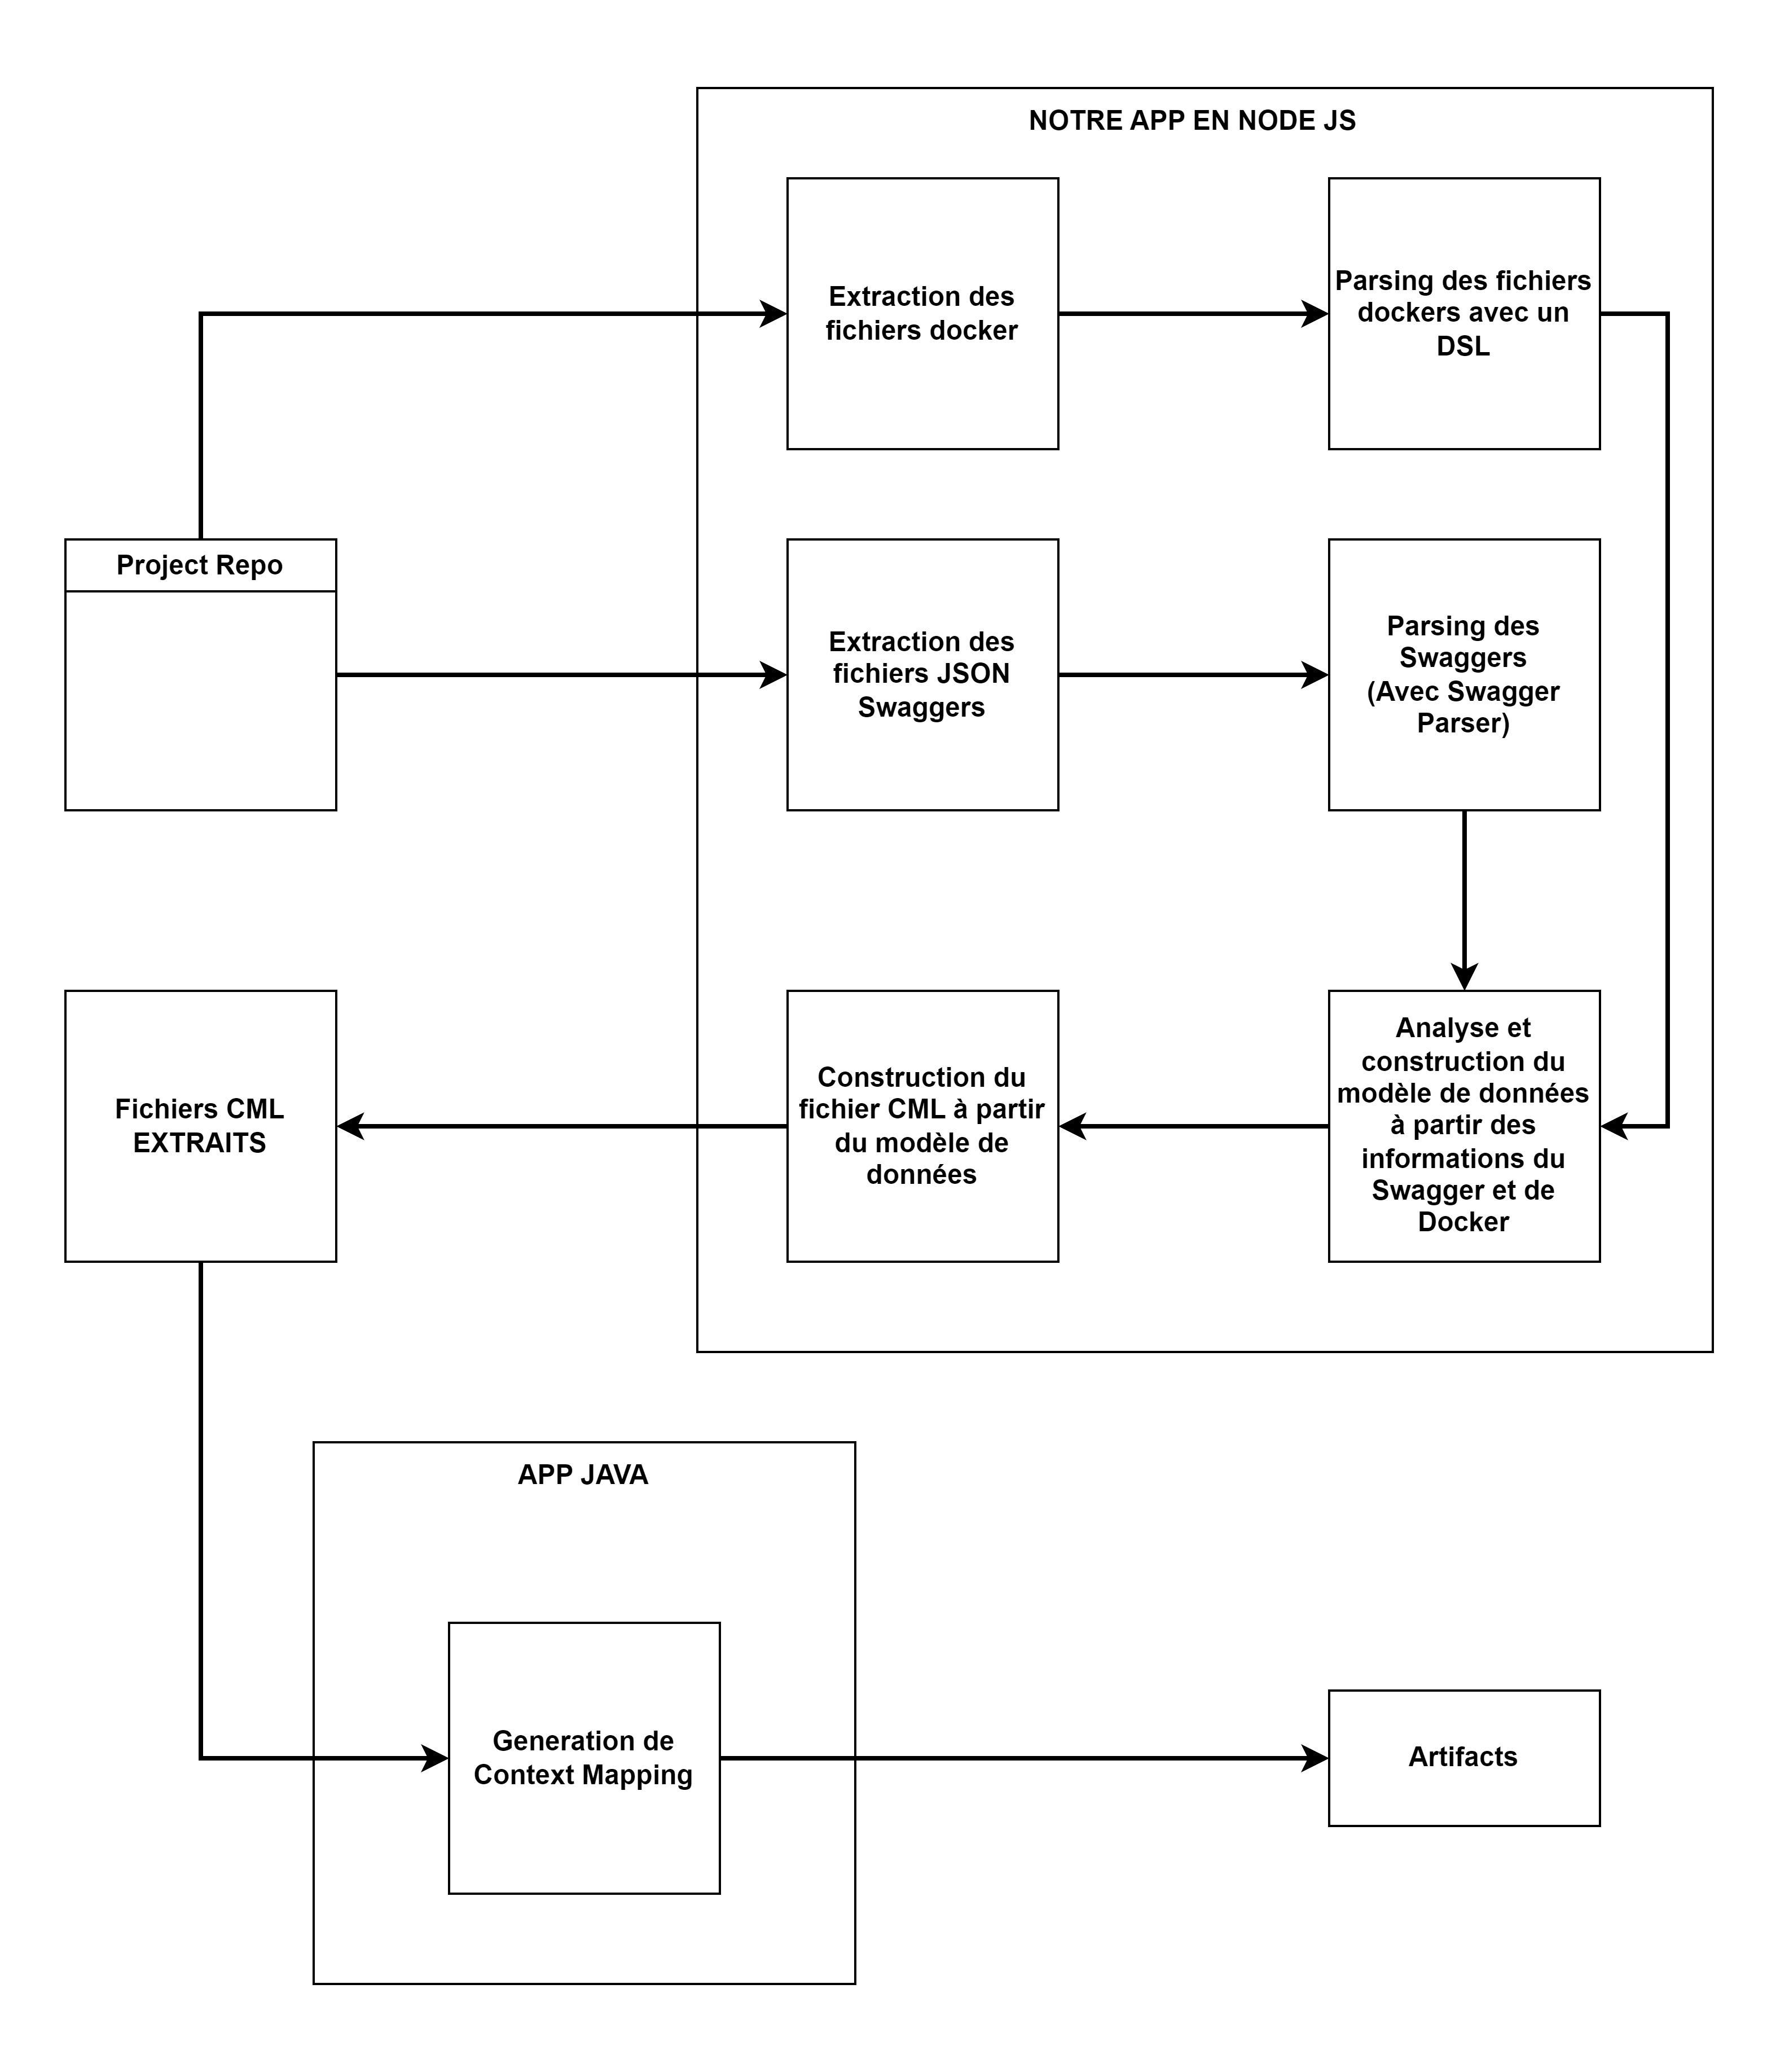
\includegraphics[width=15cm]{img/ContextMapper.png}
        \caption{Architecture prévue pour notre solution}
    \end{figure}




    \end{abstract}

    \clearpage
    \tableofcontents

    \clearpage
    \bibliographystyle{apalike-fr}
    \bibliography{biblio}
\end{document}
